\documentclass[conference]{IEEEtran}
\usepackage{cite}
\usepackage{amsmath,amssymb}
\usepackage{newtxtext,newtxmath}
\usepackage{graphicx}
\usepackage{booktabs}
\usepackage{balance}
\usepackage{array}
\usepackage{url}
\usepackage[hidelinks]{hyperref}
\graphicspath{{figures/}}

\title{Predicting 30-Day Hospital Readmission of Diabetic Patients: A Comparison of Linear, Ensemble, and Neural-Network Classifiers}
\author{\IEEEauthorblockN{Joud Tutanji, Rakan Al-Shishani, Mohammad Khalil}
\IEEEauthorblockA{Artificial Intelligence and Machine Learning Course Project}}

\begin{document}
\maketitle

\begin{abstract}
Predicting early hospital readmission from routine records is an imbalanced classification problem in which high accuracy may conceal poor detection of the patients of interest. This project compares standard classifiers on the UCI Diabetes 130-US Hospitals dataset using an evaluation procedure that keeps each patient's encounters together. After excluding death and hospice discharges, 99,343 encounters from 69,990 patients remain. Approximately 80\% of encounters are used for training and 20\% for testing, with stratified five-fold cross-validation grouped by patient within the training portion. Preprocessing is fitted inside each training fold. Seven configurations are compared: a majority baseline, ordinary and class-weighted logistic regression, a decision tree, random forest, histogram gradient boosting, and a small multilayer perceptron. Model selection uses average precision, while decision thresholds are selected from training out-of-fold predictions. Gradient boosting achieves the highest mean cross-validation average precision, 0.2334, and obtains test AUROC 0.6798, average precision 0.2386, recall 0.4593, and F1 0.2893. The majority baseline achieves 88.9\% accuracy but zero recall. The results demonstrate modest predictive discrimination and the importance of patient separation, minority-class metrics, and explicit threshold reporting. The study is an educational retrospective experiment, not a clinically validated decision system.
\end{abstract}

\begin{IEEEkeywords}
hospital readmission, diabetes, classification, class imbalance, cross-validation, scikit-learn
\end{IEEEkeywords}

\section{Introduction}
Hospital records contain information about a patient's diagnoses, treatment, laboratory testing, and previous use of healthcare services. These records provide a practical setting for studying whether standard machine-learning methods can identify encounters followed by an early readmission. The present project asks whether the information available at discharge can predict a return within 30 days. It uses the public UCI diabetes hospital dataset \cite{uci} and implements the experiment with Python and scikit-learn \cite{sklearn}.

The output is binary. An encounter labelled \texttt{<30} is positive; the labels \texttt{>30} and \texttt{NO} are combined into the negative class. This distinction matters because the task is neither diabetes diagnosis nor prediction of readmission at any future time. The intended prediction time is discharge, when the included diagnosis, medication-change, and discharge-disposition fields are available.

Two properties of the records shape the experimental design. First, early readmission is uncommon. A classifier can achieve high accuracy by predicting the majority class for every encounter. Second, some patients have multiple encounters. Splitting individual rows without grouping can place the same patient on both sides of the evaluation. Therefore, this project prioritizes patient-disjoint validation and explicitly reports positive-class performance.

The contribution is a reproducible comparison at an undergraduate course level. It combines an approximately 80/20 holdout with five-fold training cross-validation, uses small hyperparameter searches, compares class weighting within logistic regression, and examines the effect of the classification threshold. It does not introduce a new learning algorithm or assume that a complex classifier must outperform a simple one. All reported experimental results come from the completed full-data run; the smaller installation-check run is excluded from the paper.

\section{Related Work}
Strack \emph{et al.} \cite{strack} investigated HbA1c measurement and readmission using logistic regression on a filtered cohort of approximately 70,000 encounters. Their study selected one encounter per patient and provided broad diagnosis categories. The current project adapts those categories but retains repeated encounters, separating patients across training and evaluation instead of reproducing the original cohort construction.

Liu, Sue, and Wu \cite{liu} compared traditional learning methods and an LSTM on the UCI records, incorporating Grey Wolf Optimizer feature selection, SMOTE, and grouped cross-validation. Their reported AUROC values included 0.64 for XGBoost and 0.63 for random forest. Their larger feature-selection and resampling procedure is outside this project's scope.

Emi-Johnson and Nkrumah \cite{emi} used an 80/20 split and compared logistic regression, random forest, XGBoost, and a deep neural network. Reported AUROC ranged from 0.579 to 0.667. They also provided class-specific results, which help distinguish minority-class detection from aggregate accuracy. These findings motivate reporting both ranking metrics and positive-class precision, recall, and F1 here.

Saito and Rehmsmeier \cite{saito} explain why precision--recall analysis is especially useful with imbalanced labels. Accordingly, average precision (AP) is the primary model-selection criterion in this project. AUROC is retained to describe ranking performance from another perspective. AP is calculated using scikit-learn's recall-weighted definition \cite{ap}, rather than the trapezoidal area under a precision--recall curve.

Table~\ref{tab:literature} provides context only. Different cohorts, splits, preprocessing choices, and metric conventions prevent a controlled ranking of these studies. No published pipeline was reimplemented, and the current test AUROC is not evidence of superiority over those studies.

\begin{table}[t]
\caption{Same-dataset literature context; protocols are not equivalent}
\label{tab:literature}
\centering
\footnotesize
\begin{tabular}{@{}p{0.24\columnwidth}p{0.43\columnwidth}p{0.21\columnwidth}@{}}
\toprule
Study & Evaluation context & AUROC \\
\midrule
Liu et al. \cite{liu} & Grouped CV; feature selection and SMOTE & XGBoost: 0.640 \\
Emi-Johnson and Nkrumah \cite{emi} & 80/20 split; four model families & XGBoost: 0.667 \\
This project & Patient-disjoint holdout; grouped training CV & Boosting: 0.680 \\
\bottomrule
\end{tabular}
\end{table}

\section{Dataset and Preparation}
\subsection{Dataset and Target}
The source CSV contains 101,766 encounters, 47 candidate predictors, two identifiers, and one target. Its raw target counts are 11,357 for \texttt{<30}, 35,545 for \texttt{>30}, and 54,864 for \texttt{NO}. The public dataset covers care during 1999--2008 and is distributed under CC BY 4.0 \cite{uci}. Each row represents an encounter, not a unique patient.

The inputs include demographics, admission and discharge codes, diagnoses, hospital-stay measurements, previous visits, laboratory results, medication fields, and treatment summaries. Table~\ref{tab:data} summarizes the analysis cohort and the fixed split. The test portion contains 2,188 positive encounters and 17,530 negatives, giving positive prevalence 11.10\%.

\begin{table}[t]
\caption{Cohort and fixed patient-disjoint split}
\label{tab:data}
\centering
\begin{tabular}{lrr}
\toprule
Subset & Encounters & Patients \\
\midrule
Original CSV & 101,766 & 71,518 \\
Eligible cohort & 99,343 & 69,990 \\
Training & 79,625 & 55,952 \\
Testing & 19,718 & 14,038 \\
\bottomrule
\end{tabular}
\end{table}

\subsection{Eligibility and Missing Values}
Encounters with discharge codes 11, 13, 14, 19, 20, or 21 are excluded using the source mapping file. These codes represent death or hospice disposition. This removes 2,423 encounters and leaves 99,343. The rule is fixed before fitting and is applied without using the outcome to choose exclusions.

Question marks and empty cells are read as missing. In contrast, the literal value \texttt{None} in the laboratory fields is retained as ``test not performed.'' Treating it as a generic missing value would erase information about whether the laboratory test occurred. The highly incomplete \texttt{weight} field and the two documented constant drugs, \texttt{examide} and \texttt{citoglipton}, are dropped. Payer and medical-specialty fields are retained, with missing values represented by an explicit category.

Neither \texttt{encounter\_id} nor \texttt{patient\_nbr} is used as a model input. The first identifies records for auditing, while the second defines patient groups. Age remains categorical in its supplied ten-year bands. Administrative admission and discharge codes are treated as categories rather than continuous measurements.

\subsection{Feature Preparation}
Each of the three diagnosis fields is mapped to one of nine broad ICD-9 groups, with an additional category for missing diagnoses. The groups are circulatory, respiratory, digestive, diabetes, injury, musculoskeletal, genitourinary, neoplasms, and other, following the broad grouping described by Strack \emph{et al.} \cite{strack}. The mapping handles decimal codes and groups E/V codes as other.

Two simple features are added: total prior visits, the sum of prior inpatient, outpatient, and emergency visits; and number of medication changes, the count of drug fields marked \texttt{Up} or \texttt{Down}. Both are calculated from the current record. No later encounter is used to build a patient's predictors. After dropping three predictors and adding two, 46 features remain before encoding: ten numerical and 36 categorical.

Numerical features are median-imputed and standardized. Categorical features are imputed with a missing category and one-hot encoded, with unseen categories ignored at prediction time. All learned transformations are fitted inside each training pipeline. The deterministic cleaning and row-wise feature calculations do not estimate parameters from the full dataset. Exploratory summaries are produced from training records only.

\section{Experimental Methodology}
\subsection{Holdout and Cross-Validation}
A seeded \texttt{StratifiedGroupKFold} with five splits is used to construct the outer holdout. The first fold is fixed as the test set, and the other four form training. This produces 80.15\% training encounters and 19.85\% testing encounters. An exact row ratio is not required because each patient's unequal number of encounters must remain together. Stratification attempts to preserve label proportions while respecting groups \cite{groupcv}.

A separate stratified five-fold grouped splitter is then applied only to the training portion. Each training encounter appears in one validation fold. The same fold assignments are used for every model, and assertions verify zero overlap of patient IDs for the holdout and each cross-validation split. The folds are not selected according to favorable model scores.

\subsection{Models and Parameter Search}
Table~\ref{tab:models} lists the seven configurations. The majority baseline returns the training positive fraction as its score and predicts the negative class at threshold 0.5. Ordinary and balanced logistic regression share an L2-regularized model and the same two candidate values of $C$. This makes the effect of class weighting easier to inspect.

The decision tree and random forest use balanced class weights; the forest calculates them within bootstrap samples. Boosting and the MLP use the original class frequencies. Histogram gradient boosting provides an efficient scikit-learn boosting implementation without an additional learning framework. The MLP has one hidden layer containing 32 units, uses Adam with batches of 512, and trains for at most 100 epochs. Its stopping criterion uses training-loss improvement. Internal random-validation early stopping is disabled for both the MLP and boosting.

\begin{table*}[t]
\caption{Model configurations and searched settings}
\label{tab:models}
\centering
\footnotesize
\begin{tabular}{lll}
\toprule
Configuration & Fixed choices & Search \\
\midrule
Majority baseline & Training class-prior score & None \\
Logistic regression (LR) & L2; liblinear solver; maximum 1,000 iterations & $C\in\{0.1,1.0\}$ \\
Balanced LR & Same as LR; balanced class weights & $C\in\{0.1,1.0\}$ \\
Decision tree & Balanced weights; minimum leaf size 40 & Maximum depth $\in\{4,8\}$ \\
Random forest (RF) & 100 trees; minimum leaf size 10; balanced subsamples & Maximum depth $\in\{10,18\}$ \\
Histogram boosting & 100 iterations; learning rate 0.08; L2 penalty 1.0 & Maximum leaves $\in\{15,31\}$ \\
MLP & 32 hidden units; L2 penalty 0.01; learning rate 0.001 & None \\
\bottomrule
\end{tabular}
\end{table*}

Each candidate is evaluated using \texttt{GridSearchCV}, which refits the chosen configuration on the full training portion. Mean validation AP determines the selected configuration within each family. Mean CV AP also determines the overall selected model. No test prediction is requested until all model choices and thresholds are fixed.

This design is deliberately smaller than the initial proposal: it uses L2-only logistic regression, class weights instead of SMOTE, scikit-learn histogram boosting instead of XGBoost, and an untouched holdout instead of nested cross-validation. The completed run includes neither a deep network nor an exact reproduction of another paper. These scope changes keep the comparison feasible and explainable in a bachelor's course.

\subsection{Threshold Selection}
For each selected configuration, the complete pipeline is cloned and fitted separately on each training fold. Its predictions for the corresponding validation patients are collected into one out-of-fold score vector. The threshold that maximizes positive-class F1 on this vector is selected; ties use the higher threshold. The baseline retains 0.5.

The same training folds support hyperparameter selection and threshold development. Therefore, selected CV and pooled out-of-fold results are development estimates and can be optimistic. They are not presented as unbiased nested-CV estimates. The patient-disjoint test set is the final assessment of the model selected by CV. Fold standard deviation describes variation across these folds, not a confidence interval or significance test.

\subsection{Evaluation Measures}
Let TP, FP, TN, and FN denote the four confusion-matrix counts for the positive class. Precision, recall, and F1 are
\begin{align}
P &= \frac{TP}{TP+FP}, & R &= \frac{TP}{TP+FN}, \\
F_1 &= \frac{2PR}{P+R}.
\end{align}
Accuracy is $(TP+TN)/N$, while balanced accuracy is the mean of recall and specificity. All precision, recall, and F1 values in the project refer to early readmission, rather than macro- or prevalence-weighted averages.

AUROC summarizes ranking across score thresholds. AP summarizes precision at successive recall increments:
\begin{equation}
AP = \sum_k (R_k-R_{k-1})P_k.
\end{equation}
The test positive prevalence, 0.1110, is the constant-score AP reference. The Brier score measures squared probability error:
\begin{equation}
BS = \frac{1}{N}\sum_{i=1}^{N}(p_i-y_i)^2.
\end{equation}
Lower Brier scores are better. Calibration curves compare mean predicted scores with observed positive fractions in eight quantile bins. No calibration model is fitted. Test metrics are reported at both 0.5 and the previously selected threshold.

\section{Results}
\subsection{Training Cross-Validation}
The complete experiment ran in approximately 11.3 minutes in the recorded environment and produced no model-training warnings. Table~\ref{tab:cv} shows the training CV results. Histogram boosting achieved the highest AP, $0.2334\pm0.0070$, and was selected with 15 maximum leaves. The selected logistic configurations both used $C=0.1$, while the selected tree and forest depths were 8 and 18.

\begin{table}[t]
\caption{Training CV results for the selected settings}
\label{tab:cv}
\centering
\footnotesize
\begin{tabular}{lrrr}
\toprule
Model & Mean AP & AP std. & Mean AUROC \\
\midrule
Baseline & 0.1146 & 0.0020 & 0.5000 \\
LR & 0.2166 & 0.0047 & 0.6627 \\
Balanced LR & 0.2162 & 0.0051 & 0.6638 \\
Decision tree & 0.2012 & 0.0089 & 0.6423 \\
Random forest & 0.2143 & 0.0074 & 0.6678 \\
Boosting & 0.2334 & 0.0070 & 0.6716 \\
MLP & 0.2160 & 0.0063 & 0.6598 \\
\bottomrule
\end{tabular}
\end{table}

The two logistic configurations obtained nearly identical AP, indicating that class weighting did not materially improve score ranking in this search. The single tree had lower AP than the other trained families. Random forest and the MLP did not surpass ordinary logistic regression on this primary development metric. These observations apply to the chosen small search spaces, not to every possible implementation of each family.

\subsection{Held-Out Comparison}
Table~\ref{tab:test} reports the untouched test results at validation-selected thresholds. Boosting obtained AUROC 0.6798 and AP 0.2386, compared with baseline values of 0.5000 and 0.1110. Its precision was 0.2111, recall 0.4593, and F1 0.2893. Its Brier score, 0.0932, was also the lowest among the evaluated configurations. Figure~\ref{fig:curves} shows the corresponding ROC and precision--recall curves.

\begin{table*}[t]
\caption{Holdout performance at validation-selected thresholds; positive class is readmission within 30 days}
\label{tab:test}
\centering
\footnotesize
\begin{tabular}{lrrrrrrrrr}
\toprule
Model & Threshold & AUROC & AP & Accuracy & Bal. acc. & Precision & Recall & F1 & Brier \\
\midrule
Baseline & 0.5000 & 0.5000 & 0.1110 & 0.8890 & 0.5000 & 0.0000 & 0.0000 & 0.0000 & 0.0987 \\
LR & 0.1254 & 0.6658 & 0.2167 & 0.7204 & 0.6139 & 0.1928 & 0.4771 & 0.2747 & 0.0945 \\
Balanced LR & 0.5315 & 0.6670 & 0.2163 & 0.7281 & 0.6129 & 0.1953 & 0.4648 & 0.2750 & 0.2247 \\
Decision tree & 0.5503 & 0.6490 & 0.2052 & 0.7157 & 0.6181 & 0.1934 & 0.4927 & 0.2778 & 0.2254 \\
Random forest & 0.4950 & 0.6729 & 0.2154 & 0.7389 & 0.6156 & 0.2016 & 0.4570 & 0.2798 & 0.1923 \\
Boosting & 0.1383 & 0.6798 & 0.2386 & 0.7495 & 0.6225 & 0.2111 & 0.4593 & 0.2893 & 0.0932 \\
MLP & 0.1453 & 0.6536 & 0.2163 & 0.7528 & 0.5996 & 0.1980 & 0.4027 & 0.2655 & 0.0950 \\
\bottomrule
\end{tabular}
\end{table*}

\begin{figure*}[t]
\centering
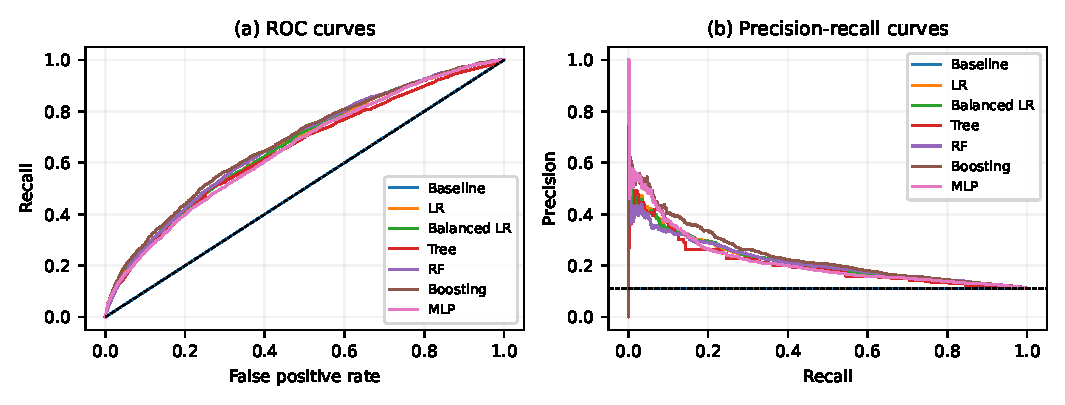
\includegraphics[width=\textwidth]{roc_pr.pdf}
\caption{Held-out ROC and precision--recall curves. The dashed precision reference is the test positive prevalence. Model and threshold selection used training data only.}
\label{fig:curves}
\end{figure*}

The baseline correctly labelled all 17,530 negative encounters but detected none of the 2,188 positives. Its accuracy of 0.8890 is therefore not evidence of useful early-readmission detection. At the chosen threshold, boosting detected 1,005 positives and missed 1,183. It also produced 3,756 false positives. This corresponds to approximately one true readmission for every 4.7 positive predictions, illustrating the remaining practical limitations despite improvement over the baseline.

\subsection{Effect of the Decision Threshold}
Table~\ref{tab:threshold} isolates the cutoff effect for the same fitted boosting model. At 0.5, it detected only 35 positive encounters, giving recall 0.0160 and F1 0.0311. Lowering the cutoff to the training-selected 0.1383 increased recall to 0.4593 and F1 to 0.2893. The tradeoff was more false positives, lower precision, and lower overall accuracy. AUROC, AP, and Brier score did not change because the underlying probability scores were unchanged.

\begin{table}[t]
\caption{Two operating points for the selected boosting model}
\label{tab:threshold}
\centering
\begin{tabular}{lrr}
\toprule
Measure & Threshold 0.5 & Threshold 0.1383 \\
\midrule
True negatives & 17,500 & 13,774 \\
False positives & 30 & 3,756 \\
False negatives & 2,153 & 1,183 \\
True positives & 35 & 1,005 \\
Precision & 0.5385 & 0.2111 \\
Recall & 0.0160 & 0.4593 \\
F1 & 0.0311 & 0.2893 \\
Accuracy & 0.8893 & 0.7495 \\
\bottomrule
\end{tabular}
\end{table}

Class weighting also changes the behavior at 0.5. Ordinary logistic regression had recall 0.0201, while balanced logistic regression had recall 0.5425. After their separately selected thresholds were applied, their recalls became 0.4771 and 0.4648, respectively, with very similar F1 scores. This demonstrates why class weighting and threshold choice should be discussed separately rather than attributing every change in recall to a different model family.

\subsection{Calibration and Feature Importance}
Figure~\ref{fig:calibration} compares raw score calibration. Balanced logistic regression and the weighted tree-based models tended to assign probabilities higher than the observed positive fractions. Balanced LR had Brier score 0.2247, compared with 0.0945 for ordinary LR. Weighting can change the probability scale even when ranking performance remains similar. These results support treating raw weighted scores cautiously and do not establish that any model is clinically calibrated.

\begin{figure}[t]
\centering
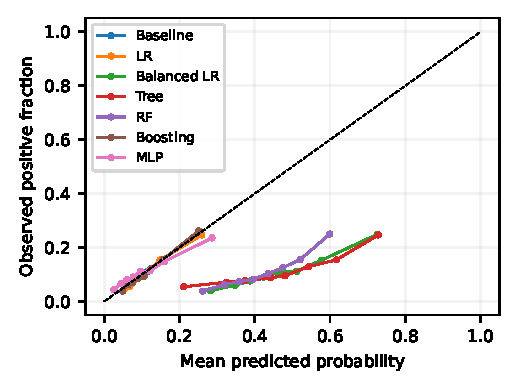
\includegraphics[width=\columnwidth]{calibration.pdf}
\caption{Quantile-binned calibration on the test set. The dashed diagonal indicates agreement between predicted probability and observed frequency.}
\label{fig:calibration}
\end{figure}

For a simple interpretation aid, Figure~\ref{fig:importance} displays the largest random-forest impurity importances. Prior inpatient visits and total prior visits ranked first and second, with importances 0.0952 and 0.0816. Laboratory procedures, medication count, discharge to home, and length of stay also appeared near the top. These are importances from the forest comparison model, not explanations of the selected boosting model. Correlated predictors can share importance, and impurity-based importance may favor variables with more possible splits. It does not identify causal effects.

\begin{figure}[t]
\centering
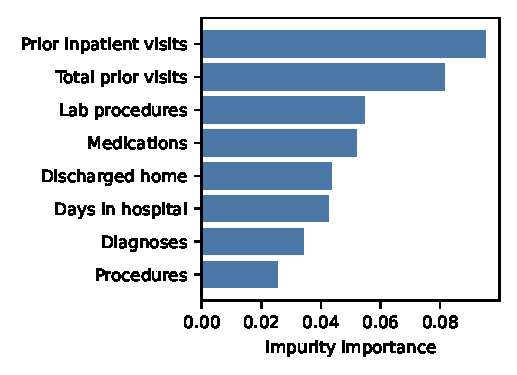
\includegraphics[width=\columnwidth]{importance.pdf}
\caption{Eight highest random-forest impurity importances, using shortened display labels.}
\label{fig:importance}
\end{figure}

\section{Discussion and Limitations}
The study shows that a manageable collection of standard classifiers can recover some readmission-related signal from the records. Boosting ranked highest in the prescribed comparison, but its test AUROC remained below 0.7 and its chosen-threshold precision was approximately 21\%. Many readmissions were missed and many flagged encounters were false alarms. These results should be described as modest predictive performance, not successful clinical deployment.

Patient separation strengthens the evaluation for patients absent from training, but does not address every generalization problem. The split is random rather than chronological, does not isolate hospitals, and does not establish performance in a future year or an external institution. The records are historical, and readmissions outside the source network may not be captured. Race, gender, and age are retained without a subgroup fairness evaluation.

Metrics weight encounters equally. A patient with several stays therefore contributes more to the reported measures than a patient with one stay, although that patient never crosses a training/test boundary. The death/hospice exclusion also defines a specific cohort; the model should not be applied as though those excluded encounters had been validated.

The small parameter grids and fixed MLP architecture limit the conclusions about model families. Reusing the training folds for both settings and threshold development can produce optimistic development scores. The independent holdout reduces this concern for the frozen selected model, but the present study reports only one holdout and no patient-bootstrap confidence intervals. Small differences between models are not claimed to be statistically significant.

Finally, F1 maximization assigns a particular balance to precision and recall; it does not represent measured costs of follow-up, missed readmissions, or clinical capacity. Choosing an operational cutoff would require separate validation and a justified decision objective. Future work could assess temporal and external generalization, subgroup performance, patient-level uncertainty estimates, calibration, and alternative imbalance methods. Those extensions are not part of the reported experiment.

\section{Implementation and Reproducibility}
The implementation separates dataset preparation, model definitions, and evaluation into three short Python modules. The main script trains all configurations, records fold and search results, fixes the selected model and thresholds, and writes test tables and figures. The saved artifact contains the fitted preprocessing pipeline, model, and chosen threshold. A companion notebook presents the workflow and completed results.

The recorded environment uses Python 3.12.3, scikit-learn 1.7.2, pandas 2.3.3, and NumPy 2.5.4. The experiment seed is 42, and the inner grouped splitter uses seed 43. Package locks, source-file checksums, split summaries, search tables, and a warning log support reproduction. Patient-level records and split-membership files remain local; the public repository contains source code, documentation, and aggregate results.

After installing the requirements, a new full run can be created with
\begin{quote}
\small\ttfamily
python run\_experiment.py --output my\_run
\end{quote}
The saved model can then be checked with
\begin{quote}
\small\ttfamily
python test\_model.py --results my\_run
\end{quote}
This check verifies the dataset checksum, loads only the held-out encounters identified by the saved split, and compares the newly calculated metrics with the recorded values. It does not refit the model or retune the threshold. Predicting a new CSV is a separate mode and, without known outcomes, does not measure accuracy.

Protocol checks cover missing values, target validation, diagnosis boundaries, identifier exclusion, patient separation, training-only transformations, and metric behavior. The original 17 checks pass after removing code comments. The test utility has also been run against the stored full-data model and a clearly labelled synthetic input record. The synthetic input demonstrates the interface and contributes no observations to the research results.

Source and supporting documentation are available at
\url{https://github.com/TheMohammadKhalil/diabetes-readmission-prediction}.

\balance
\section{Conclusion}
This project implemented a patient-disjoint comparison of standard classifiers for 30-day readmission using 99,343 eligible diabetic hospital encounters. An approximately 80/20 holdout and grouped five-fold training cross-validation produced a reproducible evaluation without sharing patients across splits. Histogram gradient boosting achieved the highest training AP and obtained test AUROC 0.6798, AP 0.2386, recall 0.4593, and F1 0.2893 at its validation-selected threshold.

The central finding is that accuracy, ranking performance, and positive-class detection describe different aspects of the task. A high-accuracy majority prediction misses every readmission, while a lower threshold finds more readmissions at the expense of false alarms. Honest reporting of these tradeoffs, together with clear separation of training and testing, is more informative than presenting a single high accuracy figure. The results support a complete course-level implementation while leaving clinical validation and broader deployment outside its claims.

\begin{thebibliography}{9}
\bibitem{uci} J. Clore, K. Cios, J. DeShazo, and B. Strack, ``Diabetes 130-US Hospitals for Years 1999--2008,'' UCI Machine Learning Repository, 2014, doi: 10.24432/C5230J.
\bibitem{sklearn} F. Pedregosa \emph{et al.}, ``Scikit-learn: Machine learning in Python,'' \emph{Journal of Machine Learning Research}, vol. 12, pp. 2825--2830, 2011.
\bibitem{strack} B. Strack, J. P. DeShazo, C. Gennings, J. L. Olmo, S. Ventura, K. J. Cios, and J. N. Clore, ``Impact of HbA1c measurement on hospital readmission rates: Analysis of 70,000 clinical database patient records,'' \emph{BioMed Research International}, vol. 2014, Art. no. 781670, 2014, doi: 10.1155/2014/781670.
\bibitem{liu} V. B. Liu, L. Y. Sue, and Y. Wu, ``Comparison of machine learning models for predicting 30-day readmission rates for patients with diabetes,'' \emph{Journal of Medical Artificial Intelligence}, vol. 7, Art. no. 23, 2024, doi: 10.21037/jmai-24-70.
\bibitem{emi} O. G. Emi-Johnson and K. J. Nkrumah, ``Predicting 30-day hospital readmission in patients with diabetes using machine learning on electronic health record data,'' \emph{Cureus}, vol. 17, no. 4, Art. no. e82437, 2025, doi: 10.7759/cureus.82437.
\bibitem{saito} T. Saito and M. Rehmsmeier, ``The precision-recall plot is more informative than the ROC plot when evaluating binary classifiers on imbalanced datasets,'' \emph{PLOS ONE}, vol. 10, no. 3, Art. no. e0118432, 2015, doi: 10.1371/journal.pone.0118432.
\bibitem{ap} Scikit-learn developers, ``average\_precision\_score,'' documentation. [Online]. Available: \url{https://scikit-learn.org/stable/modules/generated/sklearn.metrics.average_precision_score.html}. Accessed: Nov. 19, 2026.
\bibitem{groupcv} Scikit-learn developers, ``StratifiedGroupKFold,'' documentation. [Online]. Available: \url{https://scikit-learn.org/stable/modules/generated/sklearn.model_selection.StratifiedGroupKFold.html}. Accessed: Nov. 19, 2026.
\end{thebibliography}
\end{document}
